\documentclass[12pt]{article}
\usepackage[english]{babel}
\usepackage[utf8]{inputenc}
\usepackage{listings}
\usepackage[margin=1in]{geometry}
\usepackage{float}
\usepackage{amsmath}
\usepackage{graphicx} 
\usepackage{hyperref}
\hypersetup{
    colorlinks=true,
    linkcolor=blue,
    filecolor=magenta,      
    urlcolor=cyan,
    pdftitle={Overleaf Example},
    pdfpagemode=FullScreen,
    }

\title{FINAL PROJECT\\
\large Demo 3}
\author{Leonardo Cortés \and Marcelo Atencio \and Federico López \and Andrés Ruiz}
\date{February 2024}


\begin{document}

\maketitle

\begin{abstract}
The following document presents the report of the third and final stage of the final project to be presented at the Data Science Boot Camp of 'Soy Henry'. This stage includes the selection and development of the Machine Learning model, the final development of a graphical analysis in a dashboard, as well as the implementation of the proposed KPIs and finally, the implementation of both the model and the dashboard into a single deliverable product to the final client.
\end{abstract}

\tableofcontents

\section{Feature Engineering}

In this stage, we proceed to develop a business recommendation model that, when entering a category and/or business state, can suggest to the investor the highest-rated business with the most relevant words among users, in addition to 5 other similar business recommendations.


\subsection{Sentiment Analysis}

To carry out sentiment analysis, we use the function ``sentiment\_analysis" located in our resources. This function evaluates each of the user comments and assigns a rating as follows:
\begin{itemize}
    \item Value 0 for negative comments.
    \item Value 1 for neutral comments.
    \item Value 2 for positive comments.
\end{itemize}

It is of our special interest, and especially for the investor, to reduce the information to those businesses whose score is greater than 4 and with strictly positive comments (2). This narrowed information is processed in the next stage and stored in a dataframe named ``df\_filtered".

\subsection{Minimum Distance}

To the reduced information, we proceed to divide it by states and store it in individual dataframes. Then, we execute the function ``distances", which calculates the distance for each non-tourist business with respect to the nearest tourist business. The resulting information is stored in a new dataframe. Finally, we unify all the processed information into a single table.

Since the number of records is excessive to perform the Machine Learning model, we reduce the data to a sample that allows having a minimum number of businesses for each state, category, non-null minimum distance, and number of nearby businesses less than 3. This sample is saved as ``model.parquet".

\section{Recommendation Model (ML)}

In this stage, we will develop a business recommendation model. Upon entering a category and/or business state, we will suggest to the investor the highest-rated business along with the most relevant words among users. Additionally, we will provide 5 other similar business recommendations. To perform this recommendation, we have chosen cosine similarity as a comparative model between business features.

We will define 3 functions:

\subsection{Function \texttt{find\_businesses}}

This function takes a state and optionally a business category as arguments and returns the three highest-ranked businesses with the best location that are within the specified characteristics.

For example, if we enter:
\begin{itemize}
    \item State: California
    \item Category: Pub
\end{itemize}

We will get the following information:

\begin{tabular}{|l|r|r|}
\hline
Business Name & State & Category \\
\hline
Black Diamond Tavern & California & Pub \\
Woodhouse Blending \& Brewing & California & Pub \\
MCG Service LLC & California & Pub \\
\hline
\end{tabular}

If we enter:
\begin{itemize}
    \item State: New York
    \item Category: None
\end{itemize}

We will get the following information:

\begin{tabular}{|l|r|r|}
\hline
Business Name & State & Category \\
\hline
Blue Mountain Reservation Trail Lodge & New York & Hostel \\
Rosie Dunn's Victorian Pub & New York & Pub \\
Sushi Nonaka & New York & Restaurant \\
\hline
\end{tabular}


\subsection{Function \texttt{get\_recommendations}}

This function utilizes cosine similarity and takes the name of a business (generated from the \texttt{get\_business\_info} function) as an argument and returns 5 similar businesses. It considers the variables of state, category, and the nearest non-tourist business category.

\subsection{Function \texttt{get\_business\_info}}

This function takes the name of a business as an argument and generates a word cloud based on user comments and basic business information (Name, Address, City, State, category, Nearest tourist spot, and the distance to it).

For example, if we enter:
\begin{itemize}
    \item Black Diamond Tavern"
\end{itemize}

We will get the following information:

\begin{itemize}
    \item Business Name: \textit{Black Diamond Tavern}
    \item Address: \textit{Black Diamond Tavern, 42172 Moonridge Way, Big Bear Lake, CA 92315}
    \item City: \textit{Big Bear Lake}
    \item Distance: \textit{0.839082}
    \item Nearest Tourist Business: \textit{Trails End}
    \item Tourist Category: \textit{Park}
    \item Ranking: \textit{4.100000}
\end{itemize}

Additionally, a corresponding word cloud will be generated.
\begin{figure}[H]
  \centering
  \includegraphics[width=0.7\textwidth]{wordcloud.jpeg}
  \caption{Wordcloud.}
  \label{fig: Wordcloud}
\end{figure}

Moreover, it provides recommendations given by the \texttt{get\_recommendations} function.

\begin{tabular}{|l|r|r|}
\hline
Business Name & State & Category \\
\hline
Tiburon Tavern & California & Restaurant \\
Huntsman Tavern & Nevada & Pub \\
HOB Tavern & New Jersey & Pub \\
\hline
\end{tabular}

\section{Entity-Relationship Model}

Once the tables for the relational model have been defined, we proceed to visualize both the final Entity-Relationship diagram and the Primary Keys (PK) and Foreign Keys (FK) for linkage.

\begin{figure}[H]
  \centering
  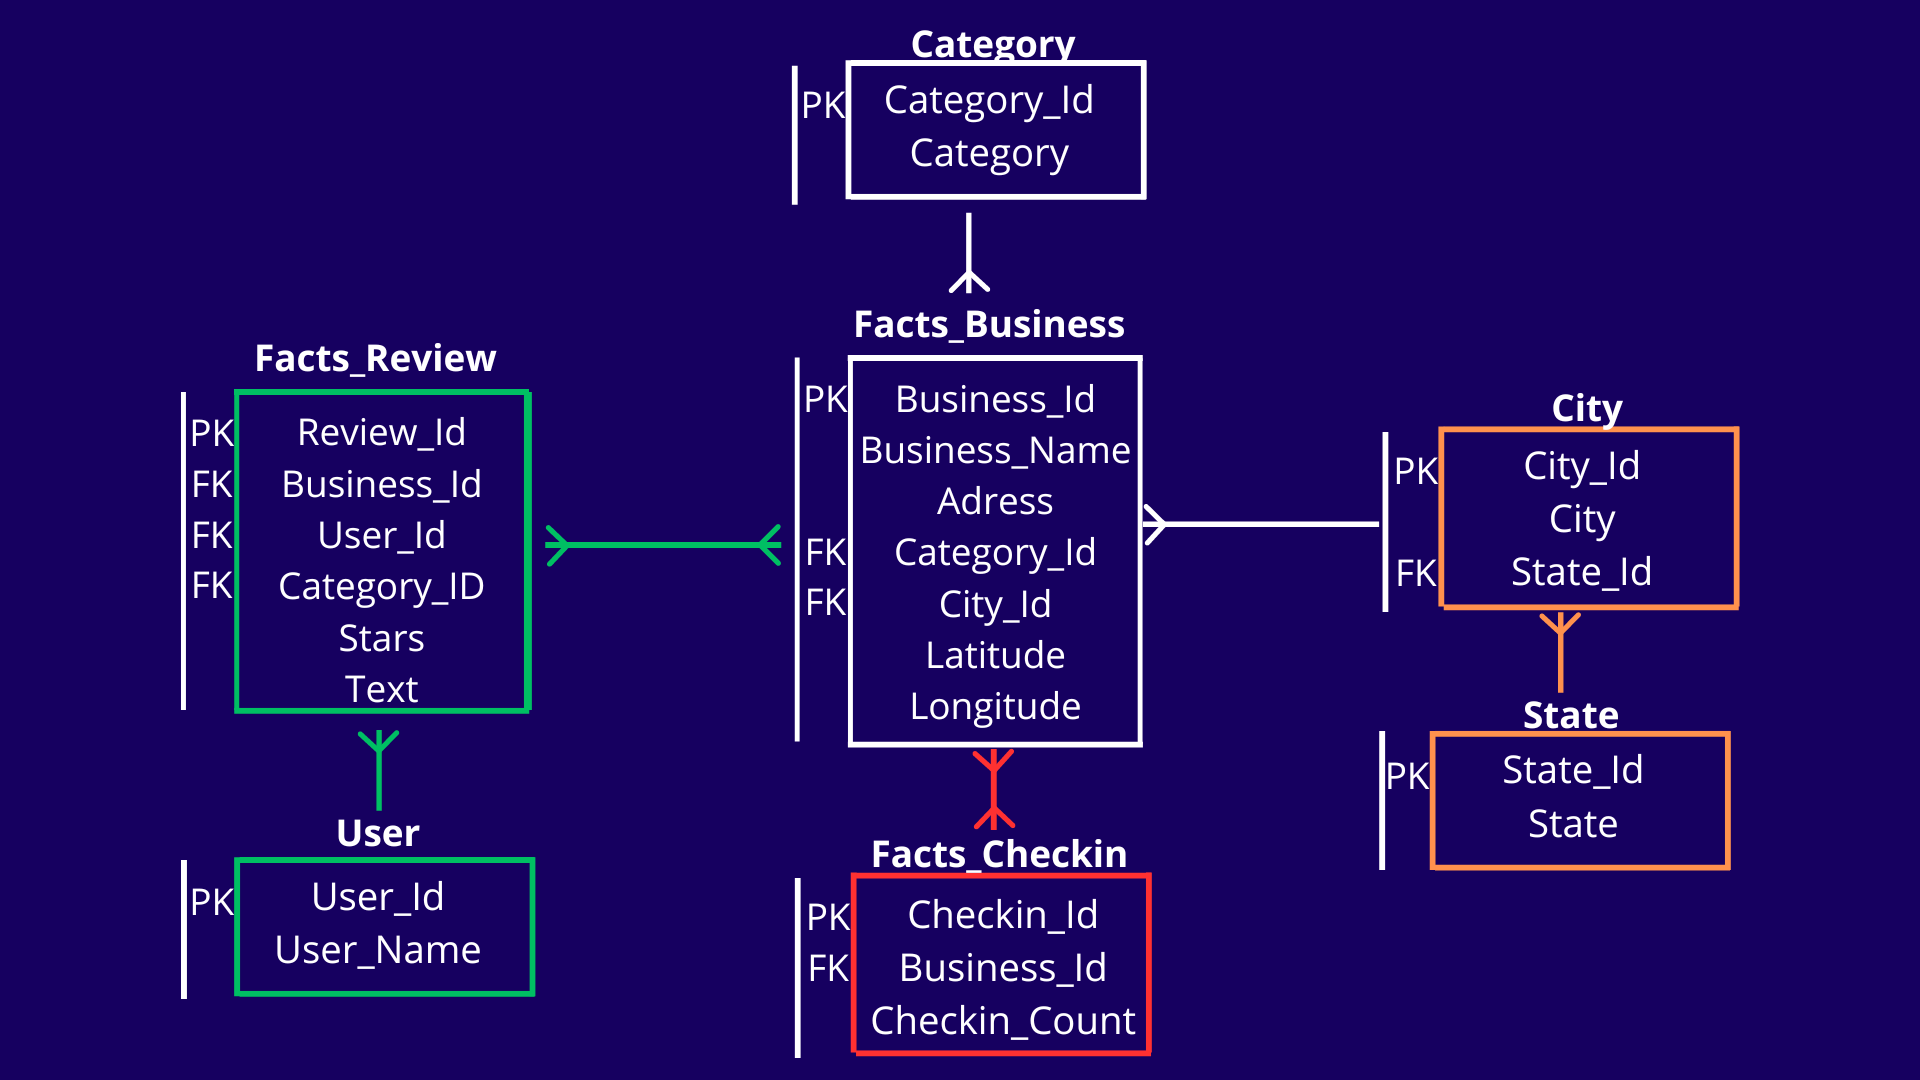
\includegraphics[width=0.7\textwidth]{DER.png}
  \caption{ERD.}
  \label{fig:ERD}
\end{figure}

Where we can see the details:
\begin{itemize}

    \item \textbf{Category Table}
    \begin{itemize}
        \item \texttt{Category\_Id}: Integer (Primary Key)
        \item \texttt{Category}: String
    \end{itemize}

    \item \textbf{City Table}
    \begin{itemize}
        \item \texttt{City\_Id}: Integer (Primary Key)
        \item \texttt{City}: String
        \item \texttt{State\_Id}: Integer (Foreign Key)
    \end{itemize}

    \item \textbf{State Table}
    \begin{itemize}
        \item \texttt{State\_Id}: Integer (Primary Key)
        \item \texttt{State}: String
    \end{itemize}

    \item \textbf{User Table}
    \begin{itemize}
        \item \texttt{User\_Id}: Object (Primary Key)
        \item \texttt{User\_Name}: Object
    \end{itemize}

    \item \textbf{Business Table}
    \begin{itemize}
        \item \texttt{Business\_Id}: Integer (Primary Key)
        \item \texttt{Business\_Name}: Object
        \item \texttt{Address}: Object
        \item \texttt{Category\_Id}: Integer (Foreign Key)
        \item \texttt{City\_Id}: Integer (Foreign Key)
        \item \texttt{Latitude}: Integer
        \item \texttt{Longitude}: Integer
    \end{itemize}

    \item \textbf{Review Table}
    \begin{itemize}
        \item \texttt{Review\_Id}: Integer (Primary Key)
        \item \texttt{Business\_Id}: Integer (Foreign Key)
        \item \texttt{Date}: Date
        \item \texttt{User\_Id}: Object (Foreign Key)
        \item \texttt{Ranking}: Integer
        \item \texttt{Stars}: Integer
        \item \texttt{Text}: Object
        \item \texttt{Sentiment\_Analysis}: Integer
    \end{itemize}

    \item \textbf{Checkin Table}
    \begin{itemize}
        \item \texttt{Checkin\_Id}: Integer (Primary Key)
        \item \texttt{Date}: Date
        \item \texttt{Business\_Id}: Integer (Foreign Key)
        \item \texttt{Checkin\_Count}: Integer
    \end{itemize}
\end{itemize}

\section{Dashboard and KPIs}

\subsection{Global Analysis}

For data visualization, we will only provide a dashboard where a global analysis of the information can be seen: business locations on the map, number of businesses by category, TOP 10 cities with the most businesses, and states with the most businesses.

\begin{figure}[H]
  \centering
  \includegraphics[width=0.8\textwidth]{analisis.png}
  \caption{Global Analysis.}
  \label{fig: Global Analysis}
\end{figure}

\subsection{Key Performance Indicators (KPIs)}

Regarding KPIs, we have determined 4 representative indicators for each business. These indicators are calculated based on a specific period and objectives are set in comparison with the previous period.

\begin{figure}[H]
  \centering
  \includegraphics[width=0.8\textwidth]{KPIs.png}
  \caption{KPIs.}
  \label{fig: KPIs}
\end{figure}

\subsection*{Online Reputation Index (ORI)}

\[ ORI = \left(\frac{\text{Number of positive reviews (SA = 2)}}{\text{Total reviews}}\right) \times 100 \]

Objective: Calculated annually, increase online reputation by 5\% compared to the previous period.

\subsection*{Customer Satisfaction Index (CSI)}

\[ CSI = \left(\frac{\text{Average user rating}}{\text{Maximum possible rating}}\right) \times 100 \]

Objective: Calculated annually, increase customer satisfaction by 10\% compared to the previous period.

\subsection*{Bad User Experience Index (BEI)}

\[ BEI = \left(\frac{\text{Number of neutral and negative reviews (SA < 2)}}{\text{Total reviews}}\right) \times 100 \]

Objective: Calculated annually, decrease bad user experience by 10\% compared to the previous period.

\subsection*{Check-In Records (CM)}

\[ CM = \text{Number of Check-Ins recorded} \]

Objective: Calculated annually, increase the number of Check-Ins recorded in the business by 5\% compared to the previous period.

The investor can select a specific business and view the indicators for the registered years, allowing them to evaluate the performance of the business over time.

\section{Final Product}

Finally, after conducting various tests with the Machine Learning model and the data used to feed the dashboard, a ``main.py" document is created containing the necessary functions to execute both the ML model and the visualization of the dashboard with the respective analysis and KPIs, all in a single deliverable final product, deploying the final result of our project through a ``web app" coded with the ``streamlit" tool. Additionally, a presentation page is created within the same app where the user can view information about the ARCOL Data Solutions team.

\begin{figure}[H]
  \centering
  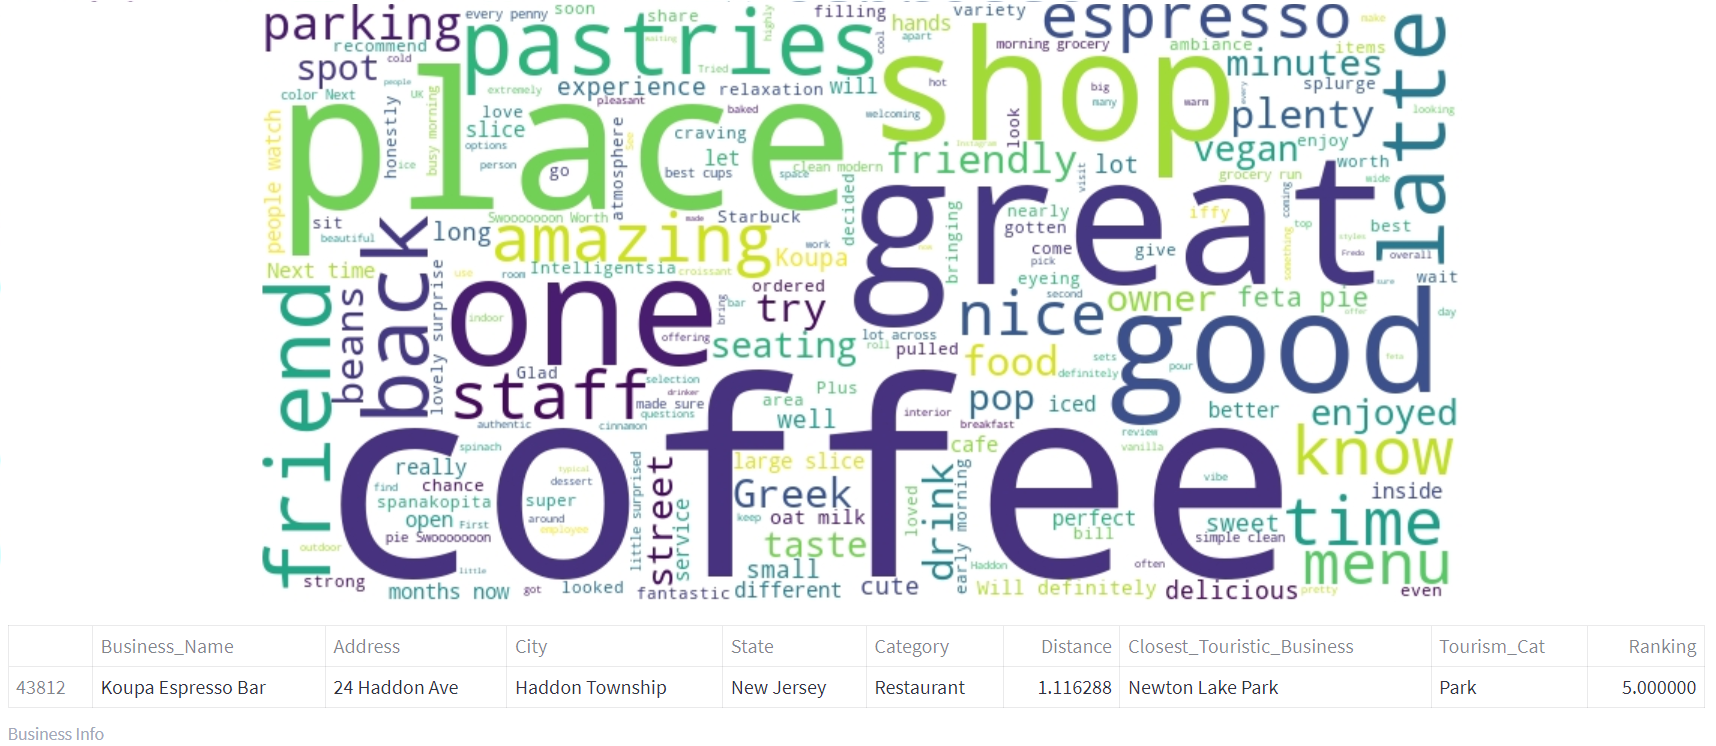
\includegraphics[width=0.8\textwidth]{ML.png}
  \caption{ML Model.}
  \label{fig: ML Model}
\end{figure}

\begin{figure}[H]
  \centering
  \includegraphics[width=0.8\textwidth]{DB.png}
  \caption{Dashboard.}
  \label{fig: Dashboard}
\end{figure}

\section{Conclusion}
In conclusion, ARCOL Data Solutions presents a comprehensive and strategic approach to the development of an investor recommendation model for the tourism sector in the United States. By leveraging the power of data analysis and machine learning techniques, we aim to provide our clients with valuable insights and actionable recommendations for making informed investment decisions. Our team of experienced professionals is committed to delivering high-quality results and exceeding client expectations. We look forward to the opportunity to collaborate with you and contribute to your success in the dynamic and competitive market landscape.

\end{document}

